\documentclass[
  man,
  longtable,
  nolmodern,
  notxfonts,
  notimes,
  colorlinks=true,linkcolor=blue,citecolor=blue,urlcolor=blue]{apa7}

\usepackage{amsmath}
\usepackage{amssymb}




\RequirePackage{longtable}
\RequirePackage{threeparttablex}

\makeatletter
\renewcommand{\paragraph}{\@startsection{paragraph}{4}{\parindent}%
	{0\baselineskip \@plus 0.2ex \@minus 0.2ex}%
	{-.5em}%
	{\normalfont\normalsize\bfseries\typesectitle}}

\renewcommand{\subparagraph}[1]{\@startsection{subparagraph}{5}{0.5em}%
	{0\baselineskip \@plus 0.2ex \@minus 0.2ex}%
	{-\z@\relax}%
	{\normalfont\normalsize\bfseries\itshape\hspace{\parindent}{#1}\textit{\addperi}}{\relax}}
\makeatother




\usepackage{longtable, booktabs, multirow, multicol, colortbl, hhline, caption, array, float, xpatch}
\setcounter{topnumber}{2}
\setcounter{bottomnumber}{2}
\setcounter{totalnumber}{4}
\renewcommand{\topfraction}{0.85}
\renewcommand{\bottomfraction}{0.85}
\renewcommand{\textfraction}{0.15}
\renewcommand{\floatpagefraction}{0.7}

\usepackage{tcolorbox}
\tcbuselibrary{listings,theorems, breakable, skins}
\usepackage{fontawesome5}

\definecolor{quarto-callout-color}{HTML}{909090}
\definecolor{quarto-callout-note-color}{HTML}{0758E5}
\definecolor{quarto-callout-important-color}{HTML}{CC1914}
\definecolor{quarto-callout-warning-color}{HTML}{EB9113}
\definecolor{quarto-callout-tip-color}{HTML}{00A047}
\definecolor{quarto-callout-caution-color}{HTML}{FC5300}
\definecolor{quarto-callout-color-frame}{HTML}{ACACAC}
\definecolor{quarto-callout-note-color-frame}{HTML}{4582EC}
\definecolor{quarto-callout-important-color-frame}{HTML}{D9534F}
\definecolor{quarto-callout-warning-color-frame}{HTML}{F0AD4E}
\definecolor{quarto-callout-tip-color-frame}{HTML}{02B875}
\definecolor{quarto-callout-caution-color-frame}{HTML}{FD7E14}

%\newlength\Oldarrayrulewidth
%\newlength\Oldtabcolsep


\usepackage{hyperref}




\providecommand{\tightlist}{%
  \setlength{\itemsep}{0pt}\setlength{\parskip}{0pt}}
\usepackage{longtable,booktabs,array}
\usepackage{calc} % for calculating minipage widths
% Correct order of tables after \paragraph or \subparagraph
\usepackage{etoolbox}
\makeatletter
\patchcmd\longtable{\par}{\if@noskipsec\mbox{}\fi\par}{}{}
\makeatother
% Allow footnotes in longtable head/foot
\IfFileExists{footnotehyper.sty}{\usepackage{footnotehyper}}{\usepackage{footnote}}
\makesavenoteenv{longtable}

\usepackage{graphicx}
\makeatletter
\newsavebox\pandoc@box
\newcommand*\pandocbounded[1]{% scales image to fit in text height/width
  \sbox\pandoc@box{#1}%
  \Gscale@div\@tempa{\textheight}{\dimexpr\ht\pandoc@box+\dp\pandoc@box\relax}%
  \Gscale@div\@tempb{\linewidth}{\wd\pandoc@box}%
  \ifdim\@tempb\p@<\@tempa\p@\let\@tempa\@tempb\fi% select the smaller of both
  \ifdim\@tempa\p@<\p@\scalebox{\@tempa}{\usebox\pandoc@box}%
  \else\usebox{\pandoc@box}%
  \fi%
}
% Set default figure placement to htbp
\def\fps@figure{htbp}
\makeatother


% definitions for citeproc citations
\NewDocumentCommand\citeproctext{}{}
\NewDocumentCommand\citeproc{mm}{%
  \begingroup\def\citeproctext{#2}\cite{#1}\endgroup}
\makeatletter
 % allow citations to break across lines
 \let\@cite@ofmt\@firstofone
 % avoid brackets around text for \cite:
 \def\@biblabel#1{}
 \def\@cite#1#2{{#1\if@tempswa , #2\fi}}
\makeatother
\newlength{\cslhangindent}
\setlength{\cslhangindent}{1.5em}
\newlength{\csllabelwidth}
\setlength{\csllabelwidth}{3em}
\newenvironment{CSLReferences}[2] % #1 hanging-indent, #2 entry-spacing
 {\begin{list}{}{%
  \setlength{\itemindent}{0pt}
  \setlength{\leftmargin}{0pt}
  \setlength{\parsep}{0pt}
  % turn on hanging indent if param 1 is 1
  \ifodd #1
   \setlength{\leftmargin}{\cslhangindent}
   \setlength{\itemindent}{-1\cslhangindent}
  \fi
  % set entry spacing
  \setlength{\itemsep}{#2\baselineskip}}}
 {\end{list}}
\usepackage{calc}
\newcommand{\CSLBlock}[1]{\hfill\break\parbox[t]{\linewidth}{\strut\ignorespaces#1\strut}}
\newcommand{\CSLLeftMargin}[1]{\parbox[t]{\csllabelwidth}{\strut#1\strut}}
\newcommand{\CSLRightInline}[1]{\parbox[t]{\linewidth - \csllabelwidth}{\strut#1\strut}}
\newcommand{\CSLIndent}[1]{\hspace{\cslhangindent}#1}





\usepackage{newtx}

\defaultfontfeatures{Scale=MatchLowercase}
\defaultfontfeatures[\rmfamily]{Ligatures=TeX,Scale=1}





\title{Chemical Conversations: Linguistic Markers of Authenticity and
Emotionality Under MDMA Influence}


\shorttitle{Chemical Conversations}


\usepackage{etoolbox}






\author{Deeksha Handa}



\affiliation{
{Social Sciences Department, University of Chicago}}




\leftheader{Handa}



\abstract{MDMA (3,4-methylenedioxymethamphetamine) has been widely
studied for its potential therapeutic effects, particularly in
facilitating emotional openness and enhancing psychotherapy outcomes.
Recent research suggests that MDMA alters speech patterns, increasing
emotional expressivity and authenticity, which may play a crucial role
in therapeutic settings. This study aims to examine the linguistic
markers of authenticity, emotionality, and fluency under the influence
of MDMA, particularly in the context of familiarity with a
conversational partner. Using a secondary analysis of data collected in
a controlled clinical setting, this study employs linguistic analysis
techniques, including the Linguistic Inquiry and Word Count (LIWC) tool,
to quantify changes in speech. Participants engaged in conversations
under four conditions---MDMA vs.~placebo and familiar vs.~unfamiliar
partner---to assess the interaction of drug effects and social context.
We hypothesize that MDMA will increase authenticity and emotional
expression with familiarity further amplifying emotional expressivity.
Understanding these linguistic shifts can provide valuable insights into
MDMA-assisted therapy (MDMA-AT), informing therapeutic approaches and
practitioner training.}

\keywords{MDMA, MDMA-AT, linguistic, LIWC}

\authornote{ 

\par{       }
\par{Correspondence concerning this article should be addressed to }
}

\makeatletter
\let\endoldlt\endlongtable
\def\endlongtable{
\hline
\endoldlt
}
\makeatother
\RequirePackage{longtable}
\DeclareDelayedFloatFlavor{longtable}{table}

\urlstyle{same}



\makeatletter
\@ifpackageloaded{caption}{}{\usepackage{caption}}
\AtBeginDocument{%
\ifdefined\contentsname
  \renewcommand*\contentsname{Table of contents}
\else
  \newcommand\contentsname{Table of contents}
\fi
\ifdefined\listfigurename
  \renewcommand*\listfigurename{List of Figures}
\else
  \newcommand\listfigurename{List of Figures}
\fi
\ifdefined\listtablename
  \renewcommand*\listtablename{List of Tables}
\else
  \newcommand\listtablename{List of Tables}
\fi
\ifdefined\figurename
  \renewcommand*\figurename{Figure}
\else
  \newcommand\figurename{Figure}
\fi
\ifdefined\tablename
  \renewcommand*\tablename{Table}
\else
  \newcommand\tablename{Table}
\fi
}
\@ifpackageloaded{float}{}{\usepackage{float}}
\floatstyle{ruled}
\@ifundefined{c@chapter}{\newfloat{codelisting}{h}{lop}}{\newfloat{codelisting}{h}{lop}[chapter]}
\floatname{codelisting}{Listing}
\newcommand*\listoflistings{\listof{codelisting}{List of Listings}}
\makeatother
\makeatletter
\makeatother
\makeatletter
\@ifpackageloaded{caption}{}{\usepackage{caption}}
\@ifpackageloaded{subcaption}{}{\usepackage{subcaption}}
\makeatother

% From https://tex.stackexchange.com/a/645996/211326
%%% apa7 doesn't want to add appendix section titles in the toc
%%% let's make it do it
\makeatletter
\xpatchcmd{\appendix}
  {\par}
  {\addcontentsline{toc}{section}{\@currentlabelname}\par}
  {}{}
\makeatother

%% Disable longtable counter
%% https://tex.stackexchange.com/a/248395/211326

\usepackage{etoolbox}

\makeatletter
\patchcmd{\LT@caption}
  {\bgroup}
  {\bgroup\global\LTpatch@captiontrue}
  {}{}
\patchcmd{\longtable}
  {\par}
  {\par\global\LTpatch@captionfalse}
  {}{}
\apptocmd{\endlongtable}
  {\ifLTpatch@caption\else\addtocounter{table}{-1}\fi}
  {}{}
\newif\ifLTpatch@caption
\makeatother

\begin{document}

\maketitle


\setcounter{secnumdepth}{-\maxdimen} % remove section numbering

\setlength\LTleft{0pt}


3,4-methylenedioxymethamphetamine (MDMA) is a synthetic drug categorized
as both a stimulant and a psychedelic, with effects comparable to
methamphetamines (\citeproc{ref-_2024_mdma}{{``{MDMA}
({Ecstasy}/{Molly}).''} 2024}). It is more commonly known as ecstasy
(pill form) and molly (crystal form). After its classification as a
Schedule I drug in 1985,unregulated research and any clinical use of
MDMA to treat psychological disorders like Post-Traumatic Stress
Disorder (PTSD) came to a sudden halt. Initial research and testing from
the 1970s had shown MDMA's potential as a less toxic,legal alternative
to MDA (3,4-methylenedioxy-amphetamine) for assisting therapy seekers
intheir emotional expression. Its clinical value centered on MDMA's
unique ability to help patients open-up emotionally, encouraging deeper
thought and introspection without overwhelming psychedelic
hallucinations. Leading therapists and scholars within the field
believed that these effects would enable otherwise hard to articulate
experiences to become easily expressible in therapeutic settings
(\citeproc{ref-passie_2018_early}{Passie, 2018}).

\subsection{Recent Clinical Developments and Methodological
Challenges}\label{recent-clinical-developments-and-methodological-challenges}

In recent years, however, 11 Phase 2 and two Phase 3 trials of
MDMA-Assisted Therapy (MDMA-AT) for PTSD treatment have been approved
and conducted. Notably, a Phase 3 trial from 2021 involved participants
receiving three MDMA doses over an 18-week period along with manualized
therapy, with significant improvement compared to placebo: over 67\% of
participants no longer met the diagnostic threshold for PTSD across a
broad range of symptoms, compared to 32\% in the placebo group
(\citeproc{ref-mitchelletal_2021_mdmaassisted}{Mitchell et al., 2021}).
Additional evidence suggests that a considerable proportion of
self-reported substance users support MDMA research (68.1\%), believe in
the potential of MDMA-assisted therapy to help with alcohol and drug
abuse Chemical Conversations 2 disorders and it's common comorbidity,
PTSD (70.1\%) and would be willing to participate if eligible (58.8\%),
across diverse racial and ethnic groups--- a previous concern in the
context of equitable distribution of MDMA-assisted therapy, given the
disproportionate extent to which substance abuse (and it's
comorbidities) affect minorities
(\citeproc{ref-jones_2023_perspectives}{Jones, 2023}). Even with these
advances, the road to MDMA-AT's broad approval and adoption is long and
complex. This is due to several concerns in the community, such as the
potential for abuse and the investment required to train therapists with
proper protocols (\citeproc{ref-maderoalvarez_2023_premise}{Madero \&
Alvarez, 2023}). Additionally, there is a concern that persistent use of
MDMA could lead to decreased cognitive function, which is a significant
argument against MDMA-AT (\citeproc{ref-wagneretal_2015_learning}{Wagner
et al., 2015}). A gaping issue here is that it is almost impossible to
construct a double-blind between placebo and MDMA conditions, given the
obvious external effects of MDMA, which could impact the results. This
exact rationale was behind the recent rejection of MDMA as a form or aid
of treatment (\citeproc{ref-kupferschmidt_2024_fda}{KUPFERSCHMIDT,
2024}). There are definite methodological advances that need to be put
in place which accurately weight the risk and benefits of such
therapeutic treatments including appropriate training and preparation
for both the therapist and the individual receiving MDMA. Wider
application for such methods will require research and analysis that
cover current gaps about our knowledge of MDMA and the experience it
induces, especially in a clinical setting with a practitioner.

\subsection{Research Gap and Thesis
formation}\label{research-gap-and-thesis-formation}

One such analysis of interest is observing and understanding overt
behavioral changes under MDMA influence, more specifically linguistic
implications, to potentially inform the construction of a therapeutic
aid. Since a critical part of PTSD therapy, like most others, involves
discussing traumatic experiences and articulating emotions,
understanding MDMA's effects on speech could deepen our knowledge of its
impact beyond general emotional facilitation. Understanding these
changes could help practitioners facilitate individuals who find it
difficult to connect with or express emotions effectively in clinical
settings. Some insights on this topic can be found in a study by Baggott
et al. (\citeproc{ref-baggottetal_2015_intimate}{2015}), which
demonstrated that MDMA alters speech content, particularly by increasing
the use of social and emotional words during discussions about intimate
relationships. The study found that MDMA enhances both positive and
negative emotional language, using a software that assesses semantic
content, the LIWC (Linguistic Inquiry and Word Count) software
(\citeproc{ref-chungpennebaker_2018_what}{Chung \& Pennebaker, 2018})
potentially helping patients in therapy communicate complex emotions
more effectively. These findings align with anecdotal reports of MDMA
encouraging emotional disclosure and suggest that MDMA may help patients
develop a language of emotional insight essential for successful trauma
processing in therapy (\citeproc{ref-baggottetal_2015_intimate}{Baggott
et al., 2015}). Further knowledge into MDMA's effects on speech are
provided in a study by Marrone et al.
(\citeproc{ref-marroneetal_2010_amphetamine}{2010}), which compared MDMA
(dose) and methamphetamine (dose) on verbal fluency and coherence. This
within-participant study showed that while methamphetamine increased
speech fluency (ability to accurately string words together) and
coherence (logical and consistent), MDMA tended to decrease fluency and
impacted participants' self-rated concentration. Movie descriptions
following MDMA were self-rated as less coherent than those after
methamphetamine, suggesting that MDMA's effects on language may differ
significantly from other amphetamines. While these studies examined
MDMA's effects on linguistic fluency and emotional language in addition
to scraping the surface with authenticity, they did so in a setting with
no direct interaction with the participant. This thesis proposes an
added variable of familiarity and unfamiliarity to an individual in the
know of the procedure, known as the confederate. Including this variable
provides a novel perspective on the research of MDMA, it may help
decipher if presence and interaction with an individual (or
practitioner) can encourage the participant even further to elucidate
their emotional state. This addition may not only help measure the
viability of the therapeutic procedure but also inform policies and
training for it. Questions of the additive nature of both MDMA and
familiarity to the individual are pertinent here.

\subsection{Research Questions and
Hypotheses}\label{research-questions-and-hypotheses}

This thesis primarily aims to identify linguistic markers of
authenticity and emotionality under the influence of MDMA to understand
the extent of MDMA-assisted therapy (MDMA- AT) in in addition to the
modulating effects of partner familiarity. To effectively examine these
aims, it is essential to first define and contextualize the primary
concepts relevant to this study: Authenticity and Emotionality.
Authenticity refers to the degree to which an individual is monitoring
their speech (LIWC --- LIWC Analysis, n.d.), while emotionality is more
about the actual words spoken and their score within LIWC.

I hypothesize that MDMA will increase linguistic markers of authenticity
and emotionality compared to placebo
(\citeproc{ref-baggottetal_2015_intimate}{Baggott et al., 2015};
\citeproc{ref-mollaetal_2023_druginduced}{Molla et al., 2023}) I expect
to seehigher authenticity and emotionality markers in conversations with
familiar partners. Familiarity can create a sense of comfort, making
speech more natural and spontaneous (LIWC --- LIWC Analysis, n.d.). On
the other hand, when interacting with an unfamiliar partner, individuals
may be more cautious about how they present themselves, leading to my
hypothesis of a decrease in authenticity and emotionality markers as
they self-monitor their language more closely.

\section{Methods}\label{methods}

This thesis project presents a secondary analysis of data from a
clinical MDMA study performed at the Human Behavioral Pharmacology Lab
by P.I. Harriet de Wit, post-doc Hanna Molla and other members of the
Lab.

\subsection{Ethical Approval}\label{ethical-approval}

This study was approved by the University of Chicago. All participants
provided informed consent to participate and were given a 250 dollars
incentive after all sessions and 50 dollars if theydropped out before
completion.

\subsection{Participants}\label{participants}

Healthy male and non-pregnant female healthy adults, aged 18 to 35, were
recruited through posters, print and internet advertisements, and
word-of-mouth referrals (n=45, f = 20; 44.5\% and m= 25; 55.5\%).
Eligible candidates were those who reported prior psychedelic use (1-40
occasions) and demonstrated verbal fluency in English. All participants
passed comprehensive medical and psychiatric screenings, including a
structured clinical interview, SCL-90R assessment, electrocardiogram,
and physical examination. Major exclusion mental and physical criteria
include previous treatment for drug or alcohol problems or current
substance dependence
(\citeproc{ref-americanpsychiatricassociation_2013_diagnostic}{American
Psychiatric Association, 2013}); past year panic disorder, history of
psychotic or manic episodes
(\citeproc{ref-americanpsychiatricassociation_2013_diagnostic}{American
Psychiatric Association, 2013}); cardiovascular illness or high
bloodpressure, abnormal EKG, and pregnancy or lactation (females).

\subsection{Procedure}\label{procedure}

Participants engaged in four laboratory sessions, conducted in random
order: Receive MDMA (100 mg) and engage in a conversation with an
Unfamiliar partner (MU), Receive placebo and engage in a conversation
with an Unfamiliar partner (PU), Receive MDMA (100 mg) and engage in a
conversation with a Familiar partner (MF), and Receive placebo and
engage in a conversation with a Familiar partner (PF).

The partners were strangers before each session, but before participants
received drug, familiarity was established with two of the partners with
a bonding conversation procedure
(\citeproc{ref-aronetal_1992_inclusion}{Aron et al., 1992},
\citeproc{ref-aronetal_1997_experimental}{1997}). One hour before
ingesting the drug or placebo, participants either engaged in a 45-min
conversation to establish familiarity with a partner (familiar
sessions), or they spent time in a room without talking (Unfamiliar
sessions).

On each session, baseline measures of heart rate, blood pressure, and
oxytocin (plasma sample were collected) were obtained, and participants
were tested for recent drug use and pregnancy. Then the participants
spent 45 minutes in the same room as their partners with or without
social interaction and filled out surveys. Following this they ingested
MDMA (100 mg) or a placebo capsule, under a double-blind condition.
Subjective measures were taken at every 30-minute mark. At the peak drug
effect (60 minutes), the confederate joined the participant for a
15-minute test conversation (which was audio recorded), this
conversation was about an important person in the participant's life
which they had already listed at the orientation. At the end of this
conversation and then the entire session, additional plasma samples were
collected. At the 240-minute mark, the participant was provided with a
snack and allowed to leave at the experimenter's discretion.

\subsection{Data Cleaning and Outcome
Measures}\label{data-cleaning-and-outcome-measures}

The main source of data in this project are the audio recordings
obtained through test conversations. These will be transcribed into text
files using Happy Scribe and human review, with dialogues from the
confederate removed. This clean text will be run through Linguistic
Inquiry and Word Count (LIWC), which is designed to count words
associated with specific psychological and grammatical dimensions to
provide quantitative data
(\citeproc{ref-chungpennebaker_2018_what}{Chung \& Pennebaker, 2018}).

For perceived authenticity, LIWC's developers categorized it as the
degree to which an individual self-monitors their speech. While high
authenticity scores can be observed in impromptu conversations between
friends, prewritten speeches tend to score lower (LIWC --- LIWC
Analysis, n.d.). This measure has been utilized by
(\citeproc{ref-markowitzetal_2023_authentic}{Markowitz et al., 2023}) in
studying the social benefits of authentic speech.

For emotional content (emotionality), LIWC analyzes both positive and
negative emotional expressions through specific word categories.
Positive emotions are tracked through words like ``good'' and ``love,''
while negative emotions are identified through terms such as ``bad'' and
``hurt.'' The analysis further breaks down negative emotions into
specific states, including anxiety (measured through words like
``worry'' and ``nervous''), anger (identified by terms such as ``mad''
and ``angry''), and sadness (tracked through words like ``cry'' and
``disappoint'').

\section{Results}\label{results}

\subsection{Data Cleaning}\label{data-cleaning}

Data preprocessing involved several steps to prepare the data for
analysis. First, string manipulation was used to extract the session
number from the \texttt{Filename} variable and create a more readable
Session label (e.g., `Session 1'). Next, the \texttt{Familiarity}
variable was refined using factor manipulation techniques. Levels were
reordered to set `Familiar' as the baseline, and less frequent levels
were grouped to simplify subsequent analyses. Finally, the
\texttt{Drugcondition} variable was recoded into a numeric
\texttt{Drugcondition\_coded} variable for statistical modeling

\subsection{Descriptive Statistics}\label{descriptive-statistics}

We began by examining the basic characteristics of our data using
descriptive statistics. Mean Authenticity and Emotion scores were
calculated overall. A custom \texttt{calculate\_mean} function was
employed to ensure accurate handling of potential missing data during
these calculations and to output those results for further tabulation
and further analysis. This approach, implemented downstream of variable
standardization, was designed to minimize risks stemming from type-based
mismatches as downstream calculations are computed and ultimately
informs appropriate test. To facilitate a comprehensive examination
across experimental groups, these key metrics were compared across drug
conditions and group size which was also constructed for sample quality,
into \textbf{Table 1}.

\begin{table}

{\caption{{Discriptive Statistics}{\label{tbl-descp}}}
\vspace{-20pt}}

\begin{longtable}[]{@{}lrlrr@{}}
\toprule\noalign{}
Drug condition & Frequency & Variable & Mean & Standard Deviation \\
\midrule\noalign{}
\endhead
\bottomrule\noalign{}
\endlastfoot
MDMA & 65 & Authenticity & 59.598308 & 20.9559477 \\
MDMA & 65 & Emotion & 1.333692 & 0.5061453 \\
placebo & 65 & Authenticity & 62.631692 & 19.0450668 \\
placebo & 65 & Emotion & 1.166923 & 0.4305517 \\
\end{longtable}

\end{table}

\vspace{-2em}

\begin{figure}

\caption{\label{fig-1}Scatter plot of Authenticity vs Familiarity by
Drug Condition}

\centering{

\pandocbounded{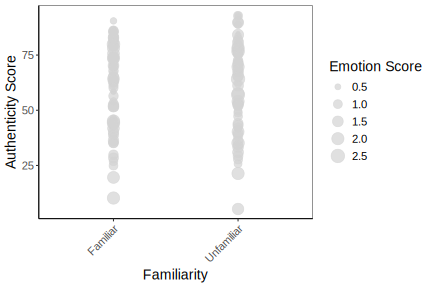
\includegraphics[keepaspectratio]{chemicalconversations_files/figure-pdf/fig-1-1.pdf}}

}

\end{figure}%

\begin{figure}

\caption{\label{fig-2}Mean Emotion Score by Drug Condition and
Familiarity}

\centering{

\pandocbounded{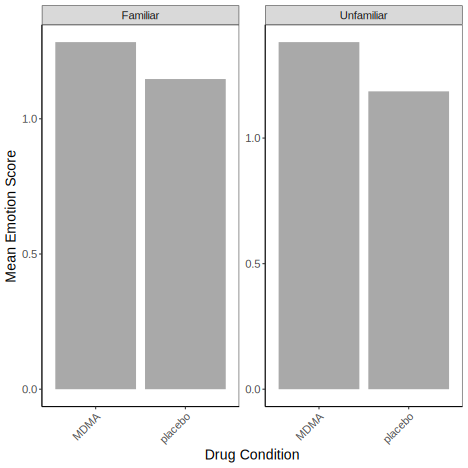
\includegraphics[keepaspectratio]{chemicalconversations_files/figure-pdf/fig-2-1.pdf}}

}

\end{figure}%

While MDMA showed slightly lower mean authenticity scores than placebo
()vs.59.6), the considerable overlap in distributions and high
variability (SDs = 20.96 for MDMA, and for Placebo) suggests individual
experiences varied widely, with some participants potentially
experiencing profound authenticity increases while others experienced
decreases. Similarly, the modest elevation in emotional response under
MDMA (1.33vs.) likely masks significant individual variation in
emotional experiences (SDs = 0.51 for MDMA, and for Placebo). Perhaps
most intriguing is the counterintuitive relationship between familiarity
and both measures, where unfamiliar stimuli consistently elicited
stronger responses across both conditions, hinting at complex
interactions between novelty, drug effects, and subjective experience.
These patterns underscore how pharmacological interventions like MDMA
may not produce uniform effects across individuals, but rather interact
with personal factors and contextual elements in ways that traditional
statistical averages may not fully capture.

\phantomsection\label{refs}
\begin{CSLReferences}{1}{0}
\bibitem[\citeproctext]{ref-americanpsychiatricassociation_2013_diagnostic}
American Psychiatric Association. (2013). \emph{Diagnostic and
{Statistical Manual} of {Mental Disorders}} (Fifth Edition). American
Psychiatric Association.
\url{https://doi.org/10.1176/appi.books.9780890425596}

\bibitem[\citeproctext]{ref-aronetal_1992_inclusion}
Aron, A., Aron, E. N., \& Smollan, D. (1992). Inclusion of {Other} in
the {Self Scale} and the structure of interpersonal closeness.
\emph{Journal of Personality and Social Psychology}, \emph{63}(4),
596--612. \url{https://doi.org/10.1037/0022-3514.63.4.596}

\bibitem[\citeproctext]{ref-aronetal_1997_experimental}
Aron, A., Melinat, E., Aron, E. N., Vallone, R. D., \& Bator, R. J.
(1997). The {Experimental Generation} of {Interpersonal Closeness}: {A
Procedure} and {Some Preliminary Findings}. \emph{Personality and Social
Psychology Bulletin}, \emph{23}(4), 363--377.
\url{https://doi.org/10.1177/0146167297234003}

\bibitem[\citeproctext]{ref-baggottetal_2015_intimate}
Baggott, M. J., Kirkpatrick, M. G., Bedi, G., \& De Wit, H. (2015).
Intimate insight: {MDMA} changes how people talk about significant
others. \emph{Journal of Psychopharmacology}, \emph{29}(6), 669--677.
\url{https://doi.org/10.1177/0269881115581962}

\bibitem[\citeproctext]{ref-chungpennebaker_2018_what}
Chung, C. K., \& Pennebaker, J. W. (2018). What {Do We Know When We
LIWC} a {Person}? {Text Analysis} as an {Assessment Tool} for {Traits},
{Personal Concerns} and {Life Stories}. In \emph{The {SAGE Handbook} of
{Personality} and {Individual Differences}: {Volume I}: {The Science} of
{Personality} and {Individual} {Differences}} (pp. 341--360). SAGE
Publications Ltd. \url{https://doi.org/10.4135/9781526451163.n16}

\bibitem[\citeproctext]{ref-jones_2023_perspectives}
Jones, J. L. (2023). Perspectives on the therapeutic potential of
{MDMA}: {A} nation-wide exploratory survey among substance users.
\emph{Frontiers in Psychiatry}, \emph{14}, 1096298.
\url{https://doi.org/10.3389/fpsyt.2023.1096298}

\bibitem[\citeproctext]{ref-kupferschmidt_2024_fda}
KUPFERSCHMIDT, K. (2024). {FDA} rejected {MDMA-assisted PTSD} therapy.
{Other} psychedelics firms intend to avoid that fate. \emph{Science}.

\bibitem[\citeproctext]{ref-maderoalvarez_2023_premise}
Madero, S., \& Alvarez, O. D. (2023). Premise, promise and challenges of
{MDMA} assisted therapy for {PTSD}. \emph{European
Neuropsychopharmacology}, \emph{70}, 19--20.
\url{https://doi.org/10.1016/j.euroneuro.2023.02.002}

\bibitem[\citeproctext]{ref-markowitzetal_2023_authentic}
Markowitz, D. M., Kouchaki, M., Gino, F., Hancock, J. T., \& Boyd, R. L.
(2023). Authentic {First Impressions Relate} to {Interpersonal},
{Social}, and {Entrepreneurial Success}. \emph{Social Psychological and
Personality Science}, \emph{14}(2), 107--116.
\url{https://doi.org/10.1177/19485506221086138}

\bibitem[\citeproctext]{ref-marroneetal_2010_amphetamine}
Marrone, G. F., Pardo, J. S., Krauss, R. M., \& Hart, C. L. (2010).
Amphetamine analogs methamphetamine and
3,4-methylenedioxymethamphetamine ({MDMA}) differentially affect speech.
\emph{Psychopharmacology}, \emph{208}(2), 169--177.
\url{https://doi.org/10.1007/s00213-009-1715-0}

\bibitem[\citeproctext]{ref-_2024_mdma}
{MDMA} ({Ecstasy}/{Molly}). (2024). \emph{NIDA}.

\bibitem[\citeproctext]{ref-mitchelletal_2021_mdmaassisted}
Mitchell, J. M., Bogenschutz, M., Lilienstein, A., Harrison, C.,
Kleiman, S., Parker-Guilbert, K., Ot'alora G., M., Garas, W., Paleos,
C., Gorman, I., Nicholas, C., Mithoefer, M., Carlin, S., Poulter, B.,
Mithoefer, A., Quevedo, S., Wells, G., Klaire, S. S., Van Der Kolk, B.,
\ldots{} Doblin, R. (2021). {MDMA-assisted} therapy for severe {PTSD}: A
randomized, double-blind, placebo-controlled phase 3 study. \emph{Nature
Medicine}, \emph{27}(6), 1025--1033.
\url{https://doi.org/10.1038/s41591-021-01336-3}

\bibitem[\citeproctext]{ref-mollaetal_2023_druginduced}
Molla, H., Lee, R., Lyubomirsky, S., \& De Wit, H. (2023). Drug-induced
social connection: Both {MDMA} and methamphetamine increase feelings of
connectedness during controlled dyadic conversations. \emph{Scientific
Reports}, \emph{13}(1), 15846.
\url{https://doi.org/10.1038/s41598-023-43156-0}

\bibitem[\citeproctext]{ref-passie_2018_early}
Passie, T. (2018). The early use of {MDMA} ({``{Ecstasy}''}) in
psychotherapy (1977--1985). \emph{Drug Science, Policy and Law},
\emph{4}, 2050324518767442.
\url{https://doi.org/10.1177/2050324518767442}

\bibitem[\citeproctext]{ref-wagneretal_2015_learning}
Wagner, D., Tkotz, S., Koester, P., Becker, B., Gouzoulis-Mayfrank, E.,
\& Daumann, J. (2015). Learning, {Memory}, and {Executive Function} in
{New MDMA Users}: {A} 2-{Year Follow-Up Study}. \emph{Frontiers in
Neuroscience}, \emph{9}. \url{https://doi.org/10.3389/fnins.2015.00445}

\end{CSLReferences}






\end{document}
